\begin{figure}[t]
\centerline{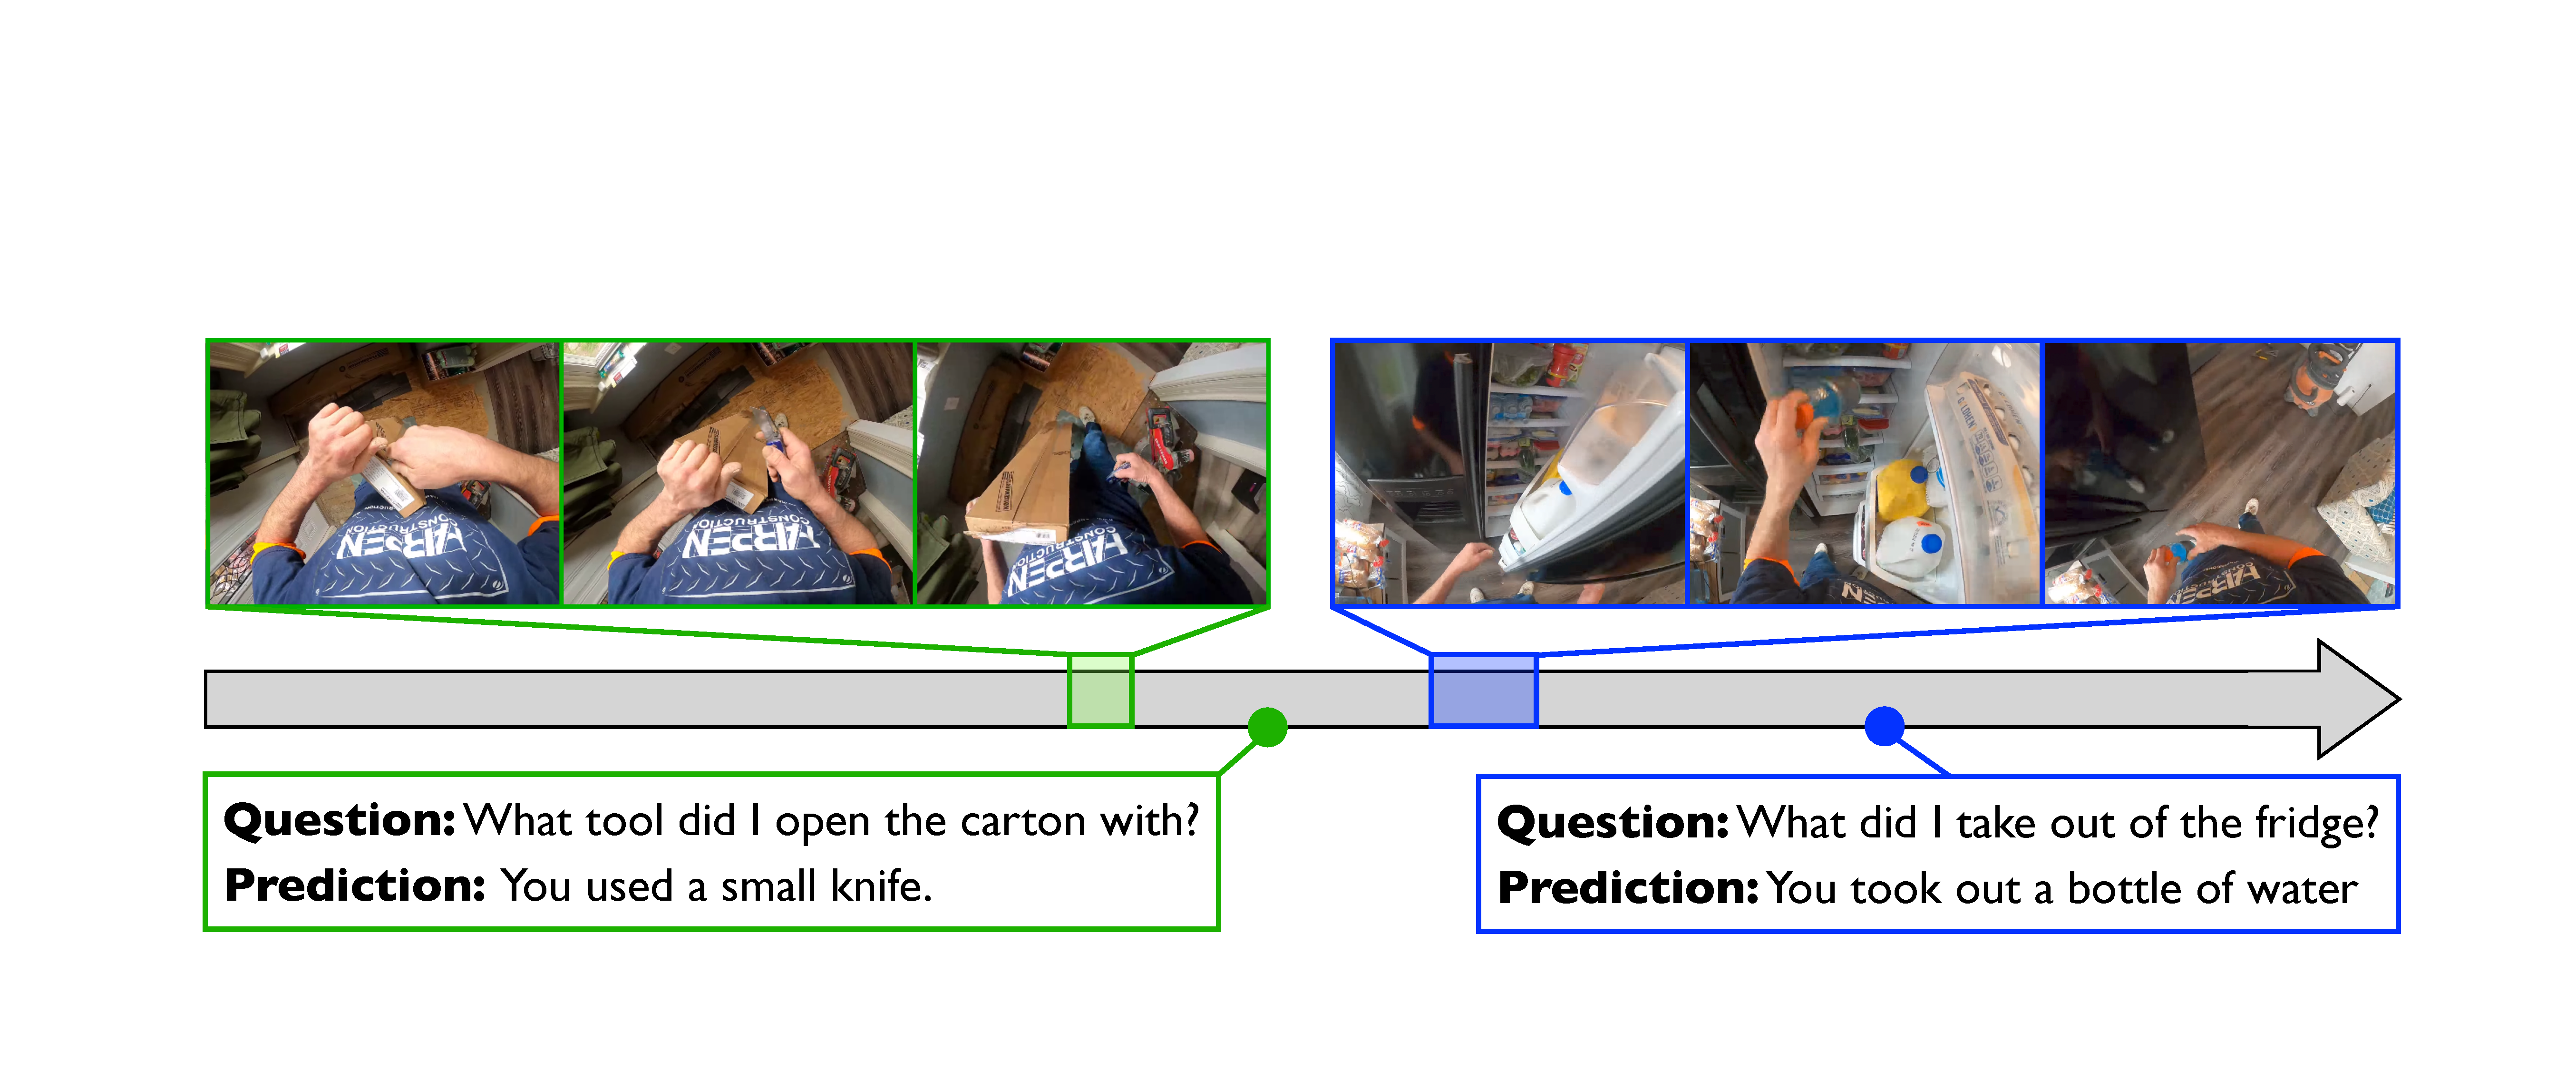
\includegraphics[width=\linewidth]{figures/src/visualization.pdf}}
\caption{
\textbf{Ejemplos cualitativos de StreamingVQA.}
El ejemplo se toma del benchmark \textsc{QaEgo4D}.
El flujo de video se procesa frame por frame.
\textcolor[RGB]{35,166,8}{$\CIRCLE$} y \textcolor{blue}{$\CIRCLE$} marcan los timestamps en los que se plantean las preguntas.
\textcolor[RGB]{35,166,8}{$\square$} y \textcolor{blue}{$\square$} indican los contextos de video relevantes que respaldan la respuesta a estas preguntas.
}
\label{fig:visualization}
\end{figure}
